\documentclass[crop=false]{standalone}
%\documentclass{standalone}
\usepackage{tikz} % To generate the plot from csv
\usepackage{pgfplots}
\usepackage{graphicx}
\usepackage{booktabs}
\usepackage{subfig}
\usepackage{float}
\usepackage[section]{placeins} % getting figures below sections
\usepackage{blindtext}
\usepackage{siunitx}
\usepgfplotslibrary{units} % Allows to enter the units nicely
\usetikzlibrary{external} %https://tex.stackexchange.com/questions/1460/script-to-automate-externalizing-tikz-graphics
\tikzexternalize[prefix=savedfigures/]

\pgfplotsset{compat=newest} % Allows to place the legend below plot
\usepackage{pgfplotstable}
\usepgfplotslibrary{statistics}

% #################### Function definition for box plots read table ##################\
\makeatletter
\pgfplotsset{
	boxplot prepared from table/.code={
		\def\tikz@plot@handler{\pgfplotsplothandlerboxplotprepared}%
		\pgfplotsset{
			/pgfplots/boxplot prepared from table/.cd,
			#1,
		}
	},
	/pgfplots/boxplot prepared from table/.cd,
	table/.code={\pgfplotstablecopy{#1}\to\boxplot@datatable},
	row/.initial=0,
	make style readable from table/.style={
		#1/.code={
			\pgfplotstablegetelem{\pgfkeysvalueof{/pgfplots/boxplot prepared from table/row}}{##1}\of\boxplot@datatable
			\pgfplotsset{boxplot/#1/.expand once={\pgfplotsretval}}
		}
	},
	make style readable from table=lower whisker,
	make style readable from table=upper whisker,
	make style readable from table=lower quartile,
	make style readable from table=upper quartile,
	make style readable from table=median,
	make style readable from table=average,
	make style readable from table=lower notch,
	make style readable from table=upper notch
}
\makeatother
\begin{document}
\pgfkeys{/pgf/number format/.cd,1000 sep={\,}}

\section{10 2 Mumford0 GA Long run 20210730 171433}

% ######################## UTRP GA Long run ######################## 
\begin{figure} 
\centering 
\tikzsetnextfilename{UTRP_NSGAII_BP_long_run} 
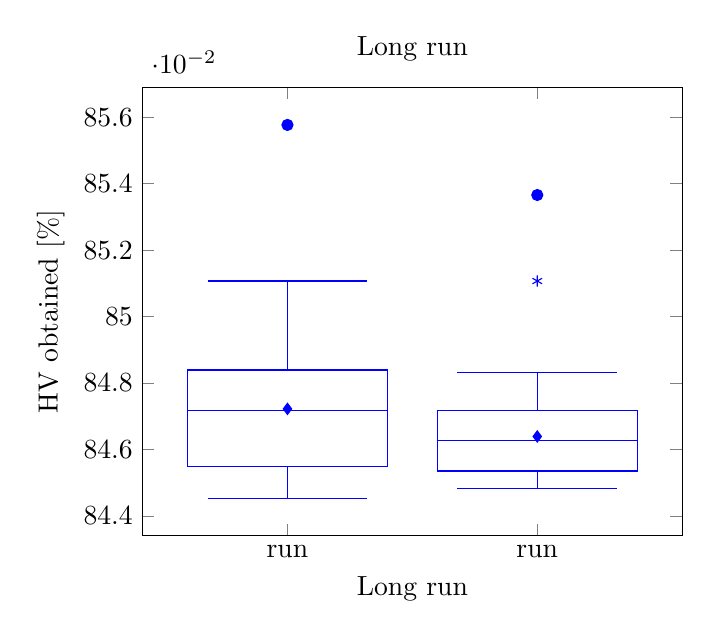
\begin{tikzpicture} 
\begin{axis}[ 
title={Long run}, 
boxplot/draw direction=y, 
xtick={1,2}, 
xticklabels={run,run}, 
x tick label style={rotate=0, align=center}, 
xlabel={Long run}, 
% y tick label style={/pgf/number format/.cd,fixed,precision=3, zerofill}, 
scaled y ticks={base 10:2}, 
ylabel={HV obtained [\%]}, 
] 

% ############## Long_run=run ################## 
\addplot[boxplot, mark=asterisk, 
boxplot prepared={ 
lower whisker=0.84452, 
upper whisker=0.85107, 
lower quartile=0.84549, 
upper quartile=0.84839, 
median=0.84717, 
average=0.84722}, 
color = blue, solid, area legend] 
coordinates {}; 
\addplot[only marks,mark=*,color = blue]coordinates{(1,0.85577)}; 

% ############## Long_run=run ################## 
\addplot[boxplot, mark=asterisk, 
boxplot prepared={ 
lower whisker=0.84482, 
upper whisker=0.84832, 
lower quartile=0.84535, 
upper quartile=0.84716, 
median=0.84626, 
average=0.84639}, 
color = blue, solid, area legend] 
coordinates {
(2,0.85107)}; 
\addplot[only marks,mark=*,color = blue]coordinates{(2,0.85366)}; 

\end{axis}
\end{tikzpicture}
\end{figure} 

\end{document}
